%==============================================================================
%  Speaker-Conditioned Verification and Lexicographic Tie-Breaking for
%  Hallucination Detection in Legislative Hearings
%  1o Desafio de Dados do Instituto Kunumi - 2026  (Ideias em Rede, 1a Edicao)
%
%  Compile:  pdflatex -> bibtex -> pdflatex -> pdflatex
%==============================================================================

\documentclass[english]{desafiokunumi}

\usepackage{tikz}
\usetikzlibrary{positioning,patterns,arrows.meta}
% amsthm colide com o \openbox do newtxmath carregado pela classe; liberamos o
% nome ANTES do load (o unico conflito restante, \Bbbk, e interno a classe)
\let\openbox\undefined
\usepackage{amsthm}

% O .cls fixa os rotulos "Resumo."/"Palavras-chave:" mesmo sob a opcao [english].
% Corrigimos aqui, a partir do main.tex, sem alterar o arquivo distribuido.
\usepackage{etoolbox}
\makeatletter
\patchcmd{\maketitle}{Resumo.}{Abstract.}{}{\typeout{[aviso] rotulo Resumo nao encontrado}}
\patchcmd{\maketitle}{Palavras-chave:}{Keywords:}{}{\typeout{[aviso] rotulo Palavras-chave nao encontrado}}
\makeatother

\newtheorem{theorem}{Theorem}
\newtheorem{proposition}[theorem]{Proposition}
\newtheorem{observation}[theorem]{Observation}
\newtheorem{corollary}[theorem]{Corollary}
\newtheorem{lemma}[theorem]{Lemma}
\theoremstyle{definition}
\newtheorem{definition}[theorem]{Definition}
\newtheorem{example}[theorem]{Example}
\theoremstyle{remark}
\newtheorem{remark}[theorem]{Remark}

\newcommand{\SE}{\mathrm{SE}}
\newcommand{\WE}{\mathrm{WE}}
\newcommand{\Ind}{\mathrm{Ind}}
\newcommand{\AUC}{\mathrm{AUROC}}
\newcommand{\prel}{\preceq}
\newcommand{\lex}{\preceq_{\mathrm{lex}}}

% =============================================================================
%  METADADOS
% =============================================================================
\title{Speaker-Conditioned Verification and Lexicographic Tie-Breaking for Hallucination Detection in Legislative Hearings}

\authors{%
  Gabriel Ribeiro\textsuperscript{1}, Cau\~a Sathler\textsuperscript{2},
  Arthur Gon\c{c}alves\textsuperscript{1}, Jordan Elias\textsuperscript{3}%
}

\affiliations{%
  \textsuperscript{1}Colab Domain-Specific Foundation Models, Departamento de
  Ci\^encia da Computa\c{c}\~ao, Universidade Federal de Minas Gerais (DCC-UFMG)\\
  \textsuperscript{2}Colab Agentic AutoML for Data Science, Departamento de
  Ci\^encia da Computa\c{c}\~ao, Universidade Federal de Minas Gerais (DCC-UFMG)\\
  \textsuperscript{3}Colab SLMs for Process Automation, Universidade Federal do
  Cear\'a (UFC)\\[2pt]
  \texttt{gabriel.ribeiro@dcc.ufmg.br}, \texttt{cauasathler@ufmg.br},\\
  \texttt{afariag72@gmail.com}, \texttt{jordanelias@alu.ufc.br}%
}

\keywords{LLM judges; hallucination detection; speaker incidence; AUROC ties; lexicographic combination; PublicHearingBR}

\abstracttext{Summaries of legislative public hearings attribute opinions to named participants, and some of these attributions are not supported by what the participants actually said. We study how to detect such errors on PublicHearingBR, a dataset of Brazilian Chamber of Deputies hearings with human verdicts for every summary opinion. We first show that standard verification scores, which compare an opinion with the whole transcript and keep the best match, cannot distinguish an opinion expressed by the attributed speaker from the same opinion expressed by someone else. Features that compare the opinion with the attributed speaker's own turns raise the AUROC (the probability of ranking a hallucination above a supported opinion) from $0.57$ to $0.76$ without any model call. We then study how to add such an inexpensive detector to a committee of twelve LLM judges. Fitting a combined model degrades the committee, because a weighted sum can overturn its decisions. Using the inexpensive score only to order opinions on which the committee is tied cannot do so, and an elementary decomposition of AUROC forecasts the gain of this rule on unseen hearings. The rule improves every committee size we tested, and its gain is largest where judges are fewest: it raises each of the twelve judges individually by $0.046$ to $0.102$ AUROC (a typical judge from $0.81$ to $0.88$), and in an exploratory analysis seven judges with the rule are statistically indistinguishable from the full committee of twelve. On this dataset, a small committee with the rule therefore approaches the accuracy of a much larger one. The rule also raises the full committee from $0.926$ to $0.930$, a small gain that is stable across twenty random assignments of hearings to folds.}

\renewcommand{\arraystretch}{0.92}

\makeatletter
\renewcommand\paragraph{\@startsection{paragraph}{4}{\z@}%
  {1.5ex \@plus 0.5ex \@minus .2ex}{-1em}%
  {\normalfont\normalsize\bfseries}}
\makeatother

\captionsetup{skip=4pt}
\setlength{\intextsep}{6pt plus 2pt minus 2pt}
\setlength{\tabcolsep}{4.5pt}

% Espacamento de titulo levemente mais apertado que o da classe (12/4 e 8/3),
% para caber no limite de 15 paginas sem reduzir corpo de texto nem tabelas.
\titlespacing*{\section}{0pt}{9pt}{3pt}
\titlespacing*{\subsection}{0pt}{6pt}{2pt}

% Mesma motivacao: com 17 ambientes de teorema e 6 displays, o espacamento
% padrao ao redor deles custa quase uma pagina. Corpo de texto, tabelas e
% figuras ficam intactos.
\makeatletter
\def\thm@space@setup{\thm@preskip=3pt \thm@postskip=3pt}
\makeatother
\setlength{\abovedisplayskip}{4pt plus 2pt minus 2pt}
\setlength{\belowdisplayskip}{4pt plus 2pt minus 2pt}
\setlength{\abovedisplayshortskip}{2pt plus 1pt}
\setlength{\belowdisplayshortskip}{3pt plus 1pt}
\setlength{\textfloatsep}{9pt plus 2pt minus 2pt}

\begin{document}
\raggedbottom
\maketitle

% =============================================================================
\section{Introduction}
\label{sec:intro}

Legislative public hearings are long events with many speakers. When they are
summarised, whether by journalists or by language models, each summary
sentence usually attributes an opinion to a named participant. An opinion that
the participant did not express is a hallucination with public consequences:
it attributes words to an identifiable person. Detecting such errors requires
comparing each attributed opinion with what that person actually said.

PublicHearingBR \citep{publichearingbr} makes this problem measurable. It
contains 206 transcripts of public hearings of the Brazilian Chamber of
Deputies, a structured summary of each hearing, and a human verdict for each of
the $4{,}238$ summary opinions: 504 of them ($11.9\%$) are marked as not
supported by the transcript. The dataset also provides the verdicts of twelve
LLM judges (three prompts applied to four models); each judge is a language
model asked whether the opinion is supported, and it returns a binary vote.
We measure detection quality by the AUROC, the probability that a randomly
chosen hallucination is scored above a randomly chosen supported opinion
($0.5$ is chance and $1$ is perfect; Section~\ref{sec:auroc-pairwise}). A
single judge reaches an AUROC between $0.734$ and $0.847$, and the sum of
the twelve votes, which we compute from the released verdicts, reaches
$0.926$, the strongest result we are aware of on this task. Unless stated
otherwise, every AUROC in this paper is computed on the $3{,}630$ opinions
whose speaker could be identified in the transcript (Section~\ref{sec:dados}). Each judge call has a
cost, however, and it is not known how inexpensive signals should be used
alongside the judges.

Inexpensive detectors compare the opinion with each sentence of the
transcript, using embedding similarity or natural language inference (NLI),
and keep the best match. On this task they reach an AUROC of $0.57$
(similarity) and $0.58$ (entailment) (Section~\ref{sec:res-orador}), far below
the judges. The reason is that a
plausible hallucination is on topic: the hearing did discuss the subject, so
some sentence of the transcript resembles the opinion.

\begin{figure}[t]
\centering
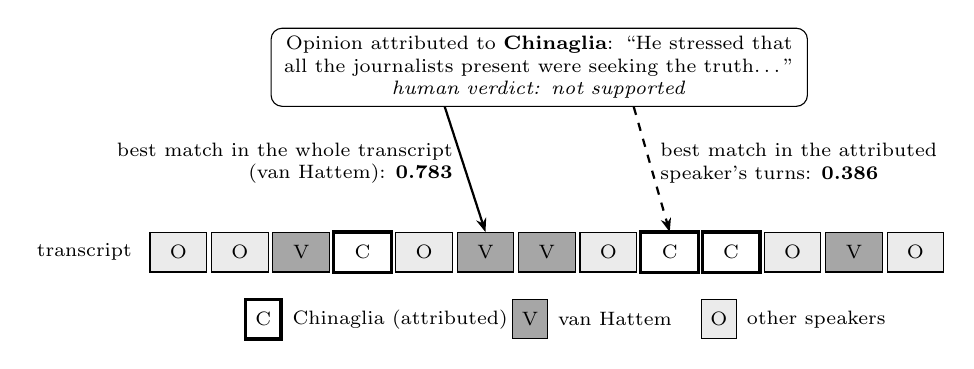
\begin{tikzpicture}[x=1cm,y=1cm,font=\scriptsize,
  seg/.style={draw,minimum height=0.5cm,minimum width=0.72cm,inner sep=0pt,anchor=west},
  arr/.style={-{Stealth[length=5pt]},thick}]
% Transcript strip (schematic order of turns): C = Chinaglia (attributed),
% V = van Hattem, O = other speakers. Scores are the measured ones.
\foreach \i/\t/\f in {0/O/black!8,1/O/black!8,2/V/black!35,3/C/white,
    4/O/black!8,5/V/black!35,6/V/black!35,7/O/black!8,8/C/white,9/C/white,
    10/O/black!8,11/V/black!35,12/O/black!8}{
  \node[seg,fill=\f] (s\i) at (\i*0.78,0) {\t};
}
\foreach \i in {3,8,9}{\draw[very thick] (s\i.south west) rectangle (s\i.north east);}
\node[anchor=east] at (-0.1,0) {transcript};
\node[draw,rounded corners,fill=white,text width=6.6cm,align=center,inner sep=3pt]
  (op) at (4.95,2.35) {Opinion attributed to \textbf{Chinaglia}: ``He stressed that
  all the journalists present were seeking the truth\ldots''\\
  \emph{human verdict: not supported}};
\draw[arr] (op.south) ++(-1.2,0) -- node[left,align=right,pos=.45]
  {best match in the whole transcript\\(van Hattem): \textbf{0.783}} (s5.north);
\draw[arr,dashed] (op.south) ++(1.2,0) -- node[right,align=left,pos=.45]
  {best match in the attributed\\speaker's turns: \textbf{0.386}} (s8.north);
% legend
\node[seg,fill=white,very thick,minimum width=0.45cm] (l1) at (1.2,-0.85) {C};
\node[anchor=west] at (l1.east) {Chinaglia (attributed)};
\node[seg,fill=black!35,minimum width=0.45cm] (l2) at (4.6,-0.85) {V};
\node[anchor=west] at (l2.east) {van Hattem};
\node[seg,fill=black!8,minimum width=0.45cm] (l3) at (7.0,-0.85) {O};
\node[anchor=west] at (l3.east) {other speakers};
\end{tikzpicture}
\caption{A real misattribution from hearing \texttt{data\_001}. The order of
turns in the strip is schematic; the two similarity scores are measured. A
score computed over the whole transcript finds strong support ($0.783$), but
that support comes from another deputy. Restricted to the attributed speaker's
turns, the best match drops to $0.386$.}
\label{fig:incidencia}
\end{figure}

Our starting observation is that the best match may belong to the wrong
person. Figure~\ref{fig:incidencia} shows a real case. In a hearing on press
freedom, the summary attributes to deputy Arlindo Chinaglia the opinion
``\emph{Destacou que todos os jornalistas presentes estavam em busca da
verdade, independentemente de suas prefer\^encias pol\'iticas}'' (``He
stressed that all the journalists present were seeking the truth, regardless
of their political preferences''), and the human annotator marked it as not
supported. The most similar sentence in the transcript has a cosine similarity
of $0.783$, but it was spoken by deputy Marcel van Hattem. The most similar
sentence among Chinaglia's own turns scores $0.386$ and concerns a different
point. A score computed over the whole transcript sees a well-supported
opinion; a score computed over the attributed speaker's turns sees an
unsupported one.

This is not a property of one example. Any score that combines sentence-level
scores through a maximum, a mean or a similar function ignores which speaker
produced each sentence, and therefore cannot separate the two situations
(Observation~\ref{prop:incidencia}). The remedy is to condition on the
speaker: we compare the opinion with the attributed speaker's turns and with
the other speakers' turns, and use these comparisons as features. We call them
\emph{speaker-incidence features}, because they use which speaker uttered
each sentence. The best match in the attributed speaker's turns alone raises
the AUROC from $0.57$ to $0.75$, and a logistic regression on all the features
reaches $0.76$, without any model call.

The second question is how to combine such a detector with the committee of
judges. The usual approach fits a model, such as a logistic regression, on
the judges' votes and the new features together. On this dataset it makes the
committee worse. The reason is structural. The committee's vote count takes
only thirteen values, so many opinions are tied, and a second detector could
usefully order them. A weighted sum, however, does more than order the ties:
it can also reverse two opinions that the committee orders correctly,
whenever the new detector disagrees strongly enough
(Proposition~\ref{prop:soma}). We instead rank opinions by the committee's
vote count and use the new detector only to order opinions that received the
same count. This \emph{lexicographic} combination never reverses a committee
decision, and its AUROC is given by an exact formula
(Proposition~\ref{thm:lex}) that depends on two quantities measurable without
running the combination: how often the committee cannot order a pair of
opinions, and how well the new detector orders those pairs.

\medskip\noindent\textbf{Contributions.}
\begin{itemize}
  \itemsep1pt
  \item Speaker-incidence features, motivated by the observation that pooled
    verification scores ignore speaker attribution, which raise AUROC by
    $0.18$ at no model cost
    (Sections~\ref{sec:teoria-incidencia} and~\ref{sec:res-orador}).
  \item A rule for combining a reliable but coarse detector with an
    inexpensive but finer one. The rule never overturns the reliable
    detector, and an elementary decomposition of AUROC gives its gain
    exactly (Section~\ref{sec:fusao}). Measured on one half of the hearings,
    the decomposition forecasts the gain on the other half without bias, at
    every committee size (Section~\ref{sec:res-escada}).
  \item A large reduction in the cost of accurate detection. The rule
    improves every committee size we tested: it raises each single judge by
    $0.046$ to $0.102$ AUROC, and in an exploratory analysis seven judges
    with the rule are statistically indistinguishable from the full
    committee of twelve (Section~\ref{sec:res-escada}).
  \item A characterisation of what remains: on the pairs of opinions that the
    committee orders incorrectly, the inexpensive detector performs below
    chance, so rules that overrule the committee when the two disagree
    cannot recover them (Section~\ref{sec:res-orcamento}).
  \item An evaluation in which predictions were committed to the repository
    before each experiment and failed predictions are reported alongside
    successful ones (Section~\ref{sec:negativos}), with all code and
    prediction files publicly
    available.\footnote{\url{https://github.com/caua-sathler/IdeiasEmRede-TopoIA}}
\end{itemize}

The paper is organised as follows. Section~\ref{sec:relacionados} reviews
related work. Section~\ref{sec:background} introduces the evaluation metric
and the notation. Section~\ref{sec:teoria} states the theoretical results.
Section~\ref{sec:dados} describes the data and the experimental protocol.
Sections~\ref{sec:res-orador} and~\ref{sec:res-fusao} report the results for
the speaker-incidence features and for their combination with the judges.
Sections~\ref{sec:negativos} and~\ref{sec:ameacas} report negative results
and threats to validity, and Section~\ref{sec:conclusao} concludes.

% =============================================================================
\section{Related Work}
\label{sec:relacionados}

\paragraph{Hallucination detection and LLM judges.}
\citet{publichearingbr} introduce the corpus, the human verdicts and the
twelve LLM-judge annotations used here. \citet{maynez2020faithfulness}
propose the standard taxonomy of faithfulness errors in abstractive
summarisation. The error our features target, content attributed to the wrong
speaker, is identified in dialogue summarisation by
\citet{ramnath2026dialsummer}, who report that LLM judges detect it only
moderately well. \citet{zheng2023judging} study the reliability of LLM judges,
including position, verbosity and self-preference biases. Our work differs in
two respects. We condition verification on the speaker to whom an opinion is
attributed, which, to our knowledge, has not been evaluated on this task. We
also treat the judges' categorical verdicts as a coarse ranking whose ties a
second detector can resolve (Section~\ref{sec:fusao}).

\paragraph{Combining detectors.} The question of when a classifier should
abstain goes back to \citet{chow1970optimum}, with the risk--coverage
formalism of \citet{elyaniv2010foundations}. A coarse detector abstains
implicitly when it assigns the same score to two items, and
Lemma~\ref{lem:contab} quantifies the effect of these ties on AUROC. Ensemble
and rank-aggregation methods usually combine scores by weighted sums. The
decomposition of AUROC into tied and separated pairs that we use is
elementary; its value is practical, since it indicates where ordering the
ties of a coarse detector can help. \citet{noh2026multillm} compare scoring the
claims of a summary jointly or independently and find the two comparable;
they vary what a scorer reads, whereas we vary how two scorers are combined.

\paragraph{Topological data analysis.} Topological methods have been applied
to hallucination detection through model internals, such as attention graphs
\citep{toha2025} and layer-wise persistence \citep{halluzig2026}. We use only
model outputs and the transcript. We also tested structural features computed
from the relation between opinions and speakers, including its homology
\citep{dowker1952homology} and a Hodge decomposition
\citep{jiang2011statistical}; they did not improve the results
(Section~\ref{sec:negativos}). The proofs in this paper use only the rankings
induced by the scores, and no property of the data or of the models, so they
hold for any primary and secondary detector and can be checked on a new
deployment by counting pairs.

% =============================================================================
\section{Background}
\label{sec:background}

This section introduces the evaluation metric and the notation used in the
rest of the paper. The definitions are standard. Lemma~\ref{lem:contab}
restates the identity of \citet{hanley1982meaning}; it is included so that the
later results can be checked, and it is not claimed as a contribution.

\subsection{AUROC as a statement about pairs}
\label{sec:auroc-pairwise}

A \emph{gold opinion} is a sentence of a structured summary attributed to a
named participant, such as the opinion attributed to deputy Chinaglia in
Figure~\ref{fig:incidencia}. A human annotator marked each opinion as supported
by the transcript or not. We call the unsupported opinions
\emph{hallucinations} (positives) and the supported ones \emph{grounded}
(negatives). A \emph{detector} is any function that assigns a real number to
each opinion, with higher values meaning more suspect. A single binary verdict
and a committee's vote count are also detectors; they simply take few distinct
values.

\begin{definition}[AUROC]
\label{def:auroc}
Let $P$ be the set of positive items, $N$ the set of negative items,
$X = P \cup N$, and $s : X \to \mathbb{R}$ a score in which larger values
indicate a positive.
Following \citet{hanley1982meaning}, who identify the area under the ROC
curve with the Mann--Whitney statistic,
\begin{equation}
  \label{eq:auroc}
  \AUC(s) \;=\; \Pr\bigl[s(p) > s(n)\bigr] \;+\; \tfrac{1}{2}\,
                \Pr\bigl[s(p) = s(n)\bigr],
\end{equation}
where $p$ and $n$ are drawn independently and uniformly from $P$ and $N$.
\end{definition}

In words, AUROC is the probability that a randomly chosen hallucination
receives a higher score than a randomly chosen grounded opinion, with ties
counted as one half. A value of $0.5$ corresponds to chance, $1.0$ to a
perfect ranking, and a value below $0.5$ to a ranking in the wrong direction.
We use AUROC rather than accuracy because positives are rare: a detector that
flags nothing is $88.1\%$ accurate yet detects nothing. AUROC is also unchanged by any
strictly increasing transformation of the score, so detectors do not need to
be calibrated. Two properties are used throughout. First, AUROC is an average
over positive--negative pairs, so it can be decomposed over any partition of
those pairs (Section~\ref{sec:res-mecanismo}). Second, the \textbf{tie
fraction} $\tau(s) = \Pr[s(p){=}s(n)]$ contributes exactly $\tau/2$.

\begin{lemma}[Tie accounting]
\label{lem:contab}
Let $A(s) = \Pr[s(p) > s(n)]$. Then $\AUC(s) = A(s) + \tau(s)/2$. Hence
$\AUC(s) \le 1 - \tau(s)/2$, with equality if and only if $s$ correctly orders
every pair it \emph{separates}, that is, every pair to which it assigns
different scores.
\end{lemma}
\begin{proof}
The identity is \eqref{eq:auroc}. Separated pairs have total probability
$1{-}\tau$, so $A \le 1{-}\tau$; substituting into the identity gives the
bound, with equality exactly when $A = 1 - \tau$, that is, when every
separated pair is ordered correctly. \qedhere
\end{proof}

\begin{remark}
\label{rem:balanced}
For a binary detector, AUROC equals the balanced accuracy,
$\tfrac12(\text{sensitivity}+\text{specificity})$, so the bound
$1 - \tau/2$ says nothing about how close a judge is to a perfect detector.
For example, a judge that flags half of the hallucinations and never flags a
grounded opinion has sensitivity $0.5$, specificity $1$ and AUROC $0.75$. It
ties every pair formed by a missed hallucination and a grounded opinion, so
$\tau = 0.5$ and the bound is $1 - \tau/2 = 0.75$: the judge attains the bound
exactly, yet misses half of the hallucinations. What the lemma provides for
any detector, binary or not, is that $\tau/2$ is the largest gain obtainable
by ordering its tied pairs while leaving the separated pairs unchanged
(Section~\ref{sec:res-fusao}).
\end{remark}

\subsection{Natural language inference}
\label{sec:bg-nli}

A \textbf{natural language inference} (NLI) model reads an ordered pair of
sentences (premise, hypothesis) and returns three probabilities:

\begin{center}\small
\begin{tabular}{@{}lll@{}}
\toprule
\textbf{label} & \textbf{meaning} & \textbf{example (premise $\to$ hypothesis)} \\
\midrule
entailment & the premise makes the hypothesis true & ``it was in 1988'' $\to$ ``it was in the 1980s'' \\
contradiction & they cannot both be true & ``it was in 1988'' $\to$ ``it was in 1995'' \\
neutral & neither of the above & ``it was in 1988'' $\to$ ``it rained that day'' \\
\bottomrule
\end{tabular}
\end{center}

Entailment is directed: ``1988'' entails ``the 1980s'', but not conversely.
Contradiction is symmetric. We use the entailment probability as a feature
(Section~\ref{sec:dados}). Each evaluation of a sentence pair is one
\emph{NLI call}.

\subsection{Pooled scores and rankings with ties}
\label{sec:bg-preorder}

Most inexpensive verification methods compute a sentence-level score
$f(o,u_i)$ between the opinion $o$ and each transcript sentence $u_i$, such as
a cosine similarity or an entailment probability, and then \emph{pool} these
scores with a maximum, a mean, or the mean of the $k$ largest values. These
pooling functions are \textbf{permutation-invariant}: their value depends only
on the collection of sentence scores, not on which sentence produced which
score. Any information that the collection does not record, such as the
speaker of each sentence, is therefore invisible to them.
Section~\ref{sec:teoria-incidencia} makes this precise.

The combination argument of Section~\ref{sec:fusao} requires one more
notion. Informally, a \emph{preorder} is a ranking that allows ties: a
committee's vote count, for instance, ranks opinions but assigns the same
value to many of them.

\begin{definition}[Preorder]
\label{def:preorder}
A relation $\preceq$ on a set is a \textbf{preorder} if it is reflexive and
transitive. Distinct items $x,y$ may satisfy $x \preceq y \preceq x$, written
$x \approx y$: they are \emph{tied}. We write $x \prec y$ when $x \preceq y$
and not $y \preceq x$ (a \emph{strict} relation). The groups of tied items are
the \textbf{equivalence classes} of the preorder. A preorder is \textbf{total}
if every two items are comparable, and it \textbf{refines} another preorder if
it keeps all the strict relations of the other and only splits some of its
ties. (These two terms are used in Proposition~\ref{thm:lex}.)
\end{definition}

A score $s$ induces the
\textbf{detector preorder} $x \preceq_s y \iff s(x) \le s(y)$. The results
below depend only on this preorder, so they are unchanged by any strictly
increasing transformation of $s$: a binary verdict and a continuous
probability are the same kind of object and differ only in the number of
equivalence classes.

\begin{example}[A committee is coarse]
\label{ex:comite}
The sum of twelve binary votes takes thirteen values. Of the $3{,}630$
opinions evaluated in Section~\ref{sec:dados}, $52.3\%$ receive zero votes,
so half of the dataset lies in a single equivalence class, within which the
committee expresses no preference. This does not imply a large tie fraction
$\tau$, because $\tau$ counts positive--negative pairs that share a class, not
items that share a class; pairs of two grounded opinions do not enter AUROC.
Only $19$ of the $408$ positives receive zero votes, against $1{,}878$
negatives, so this class contributes $19 \times 1{,}878 = 35{,}682$ tied
pairs, about $2.7\%$ of all $408 \times 3{,}222$ positive--negative pairs.
Over all thirteen classes, $\tau = 4.65\%$ (Section~\ref{sec:res-fusao},
Figure~\ref{fig:comite}).
\end{example}

\paragraph{Notation.} The symbols used in the rest of the paper are
summarised below.

\begin{center}\small
\begin{tabular}{@{}lp{0.74\linewidth}@{}}
\toprule
$P$, $N$ & positive (hallucinated) and negative (grounded) opinions \\
$s$; $s_1$, $s_2$ & a detector's score; the primary detector (the judges'
  vote count) and the secondary, inexpensive detector \\
$\tau$ & tie fraction: share of positive--negative pairs that receive equal
  scores \\
$\alpha$ & AUROC of $s_2$ restricted to the pairs that $s_1$ ties \\
$T$, $u_i$, $T_a$ & a transcript, its sentences, and the sentences spoken by
  participant $a$ \\
$\sigma$ & speaker map, assigning each sentence to its speaker \\
$\mathrm{cos}_s$, $\Delta$ & best match in the attributed speaker's turns;
  misattribution score (Section~\ref{sec:dados}) \\
$k$ & number of judges in a committee \\
\bottomrule
\end{tabular}
\end{center}

% =============================================================================
\section{Theory}
\label{sec:teoria}

\subsection{Pooled scores ignore the speaker}
\label{sec:teoria-incidencia}

Fix an opinion $o$ attributed to speaker $a$, a transcript
$T = (u_1, \dots, u_m)$ with a speaker map $\sigma : T \to \mathcal{A}$ that
assigns each sentence to the participant who uttered it, and any
sentence-level score $f(o, u_i)$.

\begin{observation}[Incidence blindness]
\label{prop:incidencia}
Any pooled score $G\bigl(\{f(o,u_i)\}_i\bigr)$, where $G$ is a maximum, a
mean, a top-$k$ mean or any other permutation-invariant function, is
invariant under every reassignment of the speaker map $\sigma$. Consequently,
no such score can distinguish an opinion supported by the turns of its
attributed speaker from the same opinion supported only by the turns of other
speakers.
\end{observation}

\begin{proof}
$G$ does not receive $\sigma$ as an argument. For a concrete separation, take
two sentences with scores $0.9$ and $0.1$. Under $\sigma_1$ the first sentence
belongs to $a$; under $\sigma_2$ it belongs to some $b \neq a$. Every pooled
$G$ takes the same value on both configurations, but only the first one
supports the opinion as attributed. \qedhere
\end{proof}

Equivalently, exchanging the speaker labels of all turns in a hearing
leaves every pooled score unchanged, although it changes the answer to the
question of whether the attributed person said what the opinion claims. No
choice of pooling function avoids this. The remedy is to pool over the
attributed speaker's sentences $T_a = \sigma^{-1}(a)$ instead of the whole
transcript, and to compare the result with the other speakers' sentences.
Section~\ref{sec:res-orador} shows that this restriction raises AUROC by
$0.18$, and that additional features describing how the support is
distributed across speakers add a smaller, significant improvement.

\subsection{Combining a coarse and a fine detector}
\label{sec:fusao}

Consider a \emph{reliable but coarse} detector $s_1$, such as the committee,
which is accurate when it separates two items but assigns the same value to
many of them, and an \emph{inexpensive but fine} detector $s_2$, which
separates almost all items but is less accurate. We call $s_1$ the
\textbf{primary} and $s_2$ the \textbf{secondary} detector throughout. The
standard way to combine them is a weighted sum, or a logistic regression on
both scores, which we call \emph{stacking}.

\begin{proposition}[A weighted sum can reverse the primary detector]
\label{prop:soma}
Let $w_1,w_2 > 0$. A pair with $x \prec_{s_1} y$ is reversed by the weighted
sum, $w_1 s_1(x) + w_2 s_2(x) > w_1 s_1(y) + w_2 s_2(y)$, if and only if
$s_2(x) - s_2(y) > (w_1/w_2)\bigl(s_1(y) - s_1(x)\bigr)$. Whenever $s_2$ is
not a non-decreasing function of $s_1$, which is the only case in which
combining the two can add information, such pairs exist once $w_2/w_1$ is
large enough.
\end{proposition}

\begin{example}[A concrete reversal]
\label{ex:witness}
Consider three opinions. Let $s_1$ be the committee's vote count divided by
twelve and $s_2$ an inexpensive score in $[0,1]$, with equal weights.
\begin{center}\small
\begin{tabular}{lccc l}
\toprule
 & $x$ & $y$ & $z$ & \\
\midrule
committee $s_1$ & $4/12$ & $5/12$ & $5/12$ & $x \prec_1 y \approx_1 z$ \\
inexpensive score $s_2$ & $0.95$ & $0.10$ & $0.90$ & \\
\midrule
sum $s_1 + s_2$ & $1.28$ & $0.52$ & $1.32$ & \textbf{reverses} $x \prec_1 y$ \\
lexicographic   & $(4,0.95)$ & $(5,0.10)$ & $(5,0.90)$ & keeps $x \prec y \prec z$ \\
\bottomrule
\end{tabular}
\end{center}
The sum ranks $x$ (four votes) above $y$ (five votes) because the inexpensive
score disagrees with the committee. The lexicographic order keeps the
committee's decision and uses $s_2$ only to separate $y$ from $z$, which the
committee could not order.
\end{example}

\begin{definition}[Lexicographic combination]
\label{def:lex}
Given detector preorders $\prel_1$ and $\prel_2$,
\begin{equation}
  \label{eq:lex}
  x \lex y \quad :\Longleftrightarrow\quad
  x \prec_1 y \quad\text{or}\quad \bigl(x \approx_1 y \ \text{and}\
  x \prel_2 y\bigr).
\end{equation}
Operationally: rank items by $s_1$, and within each group of items with equal
$s_1$, rank them by $s_2$.
\end{definition}

\begin{proposition}[Lexicographic combination]
\label{thm:lex}
$\lex$ is a total preorder containing $\prel_1 \cap \prel_2$, and
\begin{enumerate}
  \itemsep1pt
  \item[(i)] it never reverses a strict relation of $\prel_1$;
  \item[(ii)] it refines $\prel_1$ only within its equivalence classes, and
    uses no other information;
  \item[(iii)] if $\alpha$ denotes the AUROC of $s_2$ \emph{restricted to the
    positive--negative pairs that $\prel_1$ ties}, then
    \begin{equation}
      \label{eq:captura}
      \AUC(\lex) \;=\; \AUC(s_1) \;+\; \tau(s_1)\bigl(\alpha - \tfrac12\bigr)
      \qquad\text{exactly.}
    \end{equation}
    The combination therefore recovers the fraction $2\alpha - 1$ of the
    maximum possible gain $\tau/2$. It attains the full $\tau/2$ if and only
    if $\alpha = 1$, and in all cases
    $\AUC(\lex) \in [\AUC(s_1) - \tau/2,\ \AUC(s_1) + \tau/2]$.
\end{enumerate}
\end{proposition}

In words, the gain equals the share of tied pairs times how much better than
a coin flip the secondary detector orders them.

\begin{proof}
Totality and transitivity of \eqref{eq:lex} follow directly from the
definition. For the inclusion, let $x \prel_1 y$ and $x \prel_2 y$: either
$x \prec_1 y$ and the first clause applies, or $x \approx_1 y$ and the second
applies. Claim (i) is the first clause, and claim (ii) the second. For (iii),
let $A = A(s_1)$, so that $\AUC(s_1) = A + \tau/2$ by Lemma~\ref{lem:contab}.
By (i), the pairs that $s_1$ separates are ordered in the same way by $\lex$
and contribute $A$. By (ii), the tied pairs, of total probability $\tau$, are
ordered by $s_2$ alone; applying Definition~\ref{def:auroc} to this
sub-population, they contribute $\tau \alpha$ instead of $\tau/2$. Hence
$\AUC(\lex) = A + \tau \alpha$, and subtracting $\AUC(s_1)$ gives
\eqref{eq:captura}. The bound follows from $\alpha \in [0,1]$. \qedhere
\end{proof}

\begin{remark}[The gain depends on $\alpha$, not on the global AUROC of $s_2$]
\label{rem:orcamento}
The gap $1 - \tau/2 - \AUC(s_1)$ comes from pairs that $s_1$ separates in the
wrong order, and by (i) the lexicographic combination cannot change them. The
largest possible gain is therefore $\tau/2$, whatever the secondary detector.
Equation~\eqref{eq:captura} shows that, within this bound, the gain is
determined by a single number, $\alpha$, and that the global AUROC of $s_2$ does
not enter it. A candidate secondary detector should therefore be evaluated on
the primary detector's ties rather than on the whole task. The effect is
symmetric: a value of $\alpha$ below $\tfrac12$ loses exactly what the same
distance above $\tfrac12$ gains. Finally, $\tau$ depends only on the primary
detector, so the maximum gain $\tau/2$ can be computed before any secondary
detector is built; once $\alpha$ is measured on the ties,
Equation~\eqref{eq:captura} gives the gain without computing the combination.
Section~\ref{sec:res-escada} tests this as a forecast on unseen hearings.
\end{remark}

\begin{remark}[A family of combinations between the two extremes]
\label{rem:portao}
Let $r_1$ be an item's equivalence class under $\prel_1$, numbered by
consecutive integers from lowest to highest, and let $r_2 \in [0,1]$ be the
rank of $s_2$ divided by the number of items. Combine them as
$f_\gamma = r_1 + \gamma r_2$. For $0 < \gamma < 1$, $r_1(x) < r_1(y)$ implies
$f_\gamma(x) < f_\gamma(y)$, since the classes differ by at least one and
$\gamma\,|r_2(x) - r_2(y)| < 1$; within a class, $f_\gamma$ orders by $s_2$.
Hence $f_\gamma$ coincides with $\lex$. (At $\gamma = 1$, two items in
adjacent classes with $r_2 = 1$ and $r_2 = 0$ would tie.) As
$\gamma \to \infty$, $f_\gamma$ approaches the weighted sum of
Proposition~\ref{prop:soma}. The parameter $\gamma$ is thus the number of
classes of $\prel_1$ by which the secondary score may move an item. For any
$\gamma$, a pair separated by more than $\gamma$ classes can be neither
reversed nor tied, so $|\AUC(f_\gamma) - \AUC(s_1)| \le \tau/2 + \beta_\gamma$
with $\beta_\gamma = \Pr[0 < g \le \gamma]$, where $g$ is the number of classes
separating a positive--negative pair. Like $\tau$, this bound can be computed
from $s_1$ alone.
\end{remark}

% =============================================================================
\section{Data and Methods}
\label{sec:dados}

\paragraph{Data.} We use all 206 hearings of PublicHearingBR: $4{,}238$
opinions with a human verdict (504 positive, $11.9\%$) and the stored votes of
the twelve LLM judges. Sentences and opinions are embedded with multilingual
MPNet \citep{reimers2019sbert}. A \emph{turn} is a block of consecutive sentences
spoken by one participant. Turns are recovered from the transcript's speaker
markers (\texttt{O SR.\ NAME --}): each sentence is assigned to the most
recent marker. The participant named in the summary is
matched to a turn speaker by overlap of name tokens. The match succeeds for
$85.7\%$ of the opinions ($n = 3{,}630$, 408 positive), which form the main
evaluation set, since both the speaker-incidence features and the combination
experiments require the attributed speaker's turns. A failed match is itself
informative and is used as a feature in Section~\ref{sec:res-orador}.
Entailment probabilities come from mDeBERTa-v3-base-xnli
\citep{laurer2024less}.

\paragraph{Statistical protocol.} All learned models are evaluated \emph{out of fold}: we use five-fold
cross-validation in which all opinions of a hearing fall in the same fold
(\texttt{GroupKFold}), so each opinion is scored by a model fitted on other
hearings and no model is evaluated on data it was fitted on. Models are
logistic regressions with balanced class weights.
Confidence intervals resample whole hearings rather than opinions, since
opinions from the same transcript are not independent ($3{,}000$ to $5{,}000$
bootstrap resamples, depending on the analysis; all intervals are $95\%$ and, when two detectors are
compared, paired on the same resamples). Two additional sources of variance
are controlled in the combination experiments. A random tie-break is itself a
random variable, so we compare against $200$ random draws. The assignment of
hearings to folds is not captured by the bootstrap, so every combination result is
repeated over $20$ random assignments of hearings to folds (\emph{fold
partitions}) and reported as median and range. Where a single value is
reported, it comes from one representative partition. Scripts that use
different fold partitions report slightly different values for the same
quantity, for example $0.7605$ and $0.7617$ for the speaker-incidence
features, or $\alpha = 0.5856$ on the representative partition against a
median of $0.589$ over twenty partitions; such differences, in the third
decimal place, are fold noise and not different quantities. The predictions for
each experiment were committed to the repository before it was run (we call
them \emph{pre-specified}); those that failed are reported in
Section~\ref{sec:negativos}.

\paragraph{Speaker-incidence features.} For an opinion $o$ attributed to the
matched speaker $a$, let $S(o,\cdot)$ be the cosine similarity between $o$ and
each transcript sentence, $T$ the set of all sentences, and $T_a$ the set of
sentences spoken by $a$.

\begin{center}
\small
\begin{tabular}{@{}lp{0.72\linewidth}@{}}
\toprule
$\mathrm{cos}_g$ & $\max_{s \in T} S(o,s)$: best match in the whole transcript (baseline) \\
$\mathrm{cos}_s$ & $\max_{s \in T_a} S(o,s)$: best match in the attributed speaker's turns \\
$\Delta$ & $\max_{b \neq a}\max_{s \in T_b} S(o,s) - \mathrm{cos}_s$: how much
  better another speaker supports the opinion \\
$\mathrm{share}_a$ & sum of the similarities of the ten best global matches
  that lie in $T_a$, divided by their total \\
$\mathrm{rank}_a$ & rank of $a$ among all speakers ordered by their best
  match, scaled to $[0,1]$ \\
$\mathrm{cover}_a$ & $1$ if $a$ is among the strong supporters, i.e.\ the
  speakers with at least one sentence of similarity $\ge 0.65$ \\
$\mathrm{nli}_s, \mathrm{nli}_g$ & maximum entailment probability over the
  five best-matching sentences of $a$ / of the whole transcript \\
\bottomrule
\end{tabular}
\end{center}

The feature $\mathrm{cos}_s$ asks whether the attributed speaker's own turns
support the opinion, and $\Delta$ asks whether somebody else supports it
better; we call $\Delta$ the \emph{misattribution score}. When a feature is
used alone as a detector, it is oriented so that larger values indicate a
more suspect opinion (for example, $-\mathrm{cos}_s$). The remaining
features describe how much of the support belongs to the attributed speaker,
where that speaker ranks, and whether the speaker is among the supporters at
all. None of these quantities can be computed from a pooled score
(Observation~\ref{prop:incidencia}). The cosine features require no model call
beyond the precomputed embeddings; the two entailment features require ten
NLI calls per opinion.

\paragraph{The two detectors combined in Section~\ref{sec:res-fusao}.} The
primary detector $s_1 \in \{0,\dots,12\}$ is the number of judges that flag
an opinion. This unweighted vote count outperforms logistic weights fitted
out of fold on the same votes ($0.9260$ vs.\ $0.9245$ on the representative
partition, and a median of $0.9226$ over twenty partitions,
Table~\ref{tab:estab}). The secondary detector is a logistic regression on all the
speaker-incidence features, including the two NLI features ($0.7792$, ten NLI
calls per opinion); unless stated otherwise, Section~\ref{sec:res-fusao} uses
this detector. \emph{Stacking}
denotes a logistic regression fitted out of fold on the votes and the same
features together. As a control, Section~\ref{sec:res-controles}
also uses a deliberately weak inexpensive detector, $\mathrm{cos}_g$.

% =============================================================================
\section{Results I: Speaker-Incidence Features}
\label{sec:res-orador}

\subsection{Conditioning on the attributed speaker}

Table~\ref{tab:orador} reports the main result of this section. On the
$3{,}630$ matched opinions, the best match in the whole transcript reaches an
AUROC of $0.5676$ ($0.5628$ over all $4{,}238$ opinions). Computing the same
similarity over the attributed speaker's turns raises it to $0.7455$, a
difference of $+0.178$ (clustered CI $[+0.128, +0.237]$).

\begin{table}[!ht]
  \centering
  \caption{AUROC of each signal against the human verdict on the
  matched-speaker subset ($n=3{,}630$, 408 positives). ``0 calls'' means the
  signal is computed from precomputed embeddings and speaker markers alone.}
  \label{tab:orador}
  \small
  \begin{tabular}{@{}llc@{}}
    \toprule
    \textbf{Signal} & \textbf{Cost / opinion} & \textbf{AUROC} \\
    \midrule
    $\mathrm{cos}_g$: best match in the whole transcript (baseline) & 0 calls & 0.5676 \\
    $\mathrm{nli}_g$: best entailment in the whole transcript (baseline) & $\sim$10 NLI & 0.5828 \\
    \midrule
    $\mathrm{cos}_s$: \textbf{best match in the attributed speaker's turns} & 0 calls & \textbf{0.7455} \\
    $\Delta$: misattribution score                                & 0 calls & 0.7595 \\
    $\mathrm{share}_a$: share of the support                     & 0 calls & 0.7135 \\
    $\mathrm{rank}_a$: rank of the speaker                       & 0 calls & 0.7258 \\
    $\mathrm{cover}_a$: speaker among strong supporters          & 0 calls & 0.6706 \\
    \textbf{all speaker-incidence features, out of fold}          & 0 calls & \textbf{0.7605} \\
    all features $+$ $\mathrm{nli}_s, \mathrm{nli}_g$            & $\sim$10 NLI & \textbf{0.7792} \\
    \bottomrule
  \end{tabular}
\end{table}

Three controls address alternative explanations.
\textbf{Speaker identity.} Computing the same feature over a \emph{randomly
chosen other} speaker of the same hearing, matched for number of turns, gives
$0.5209$, which is at chance and below the global baseline. The paired
difference between the attributed and the random speaker is $+0.2246$
$[+0.1903, +0.2592]$, so the signal comes from \emph{who} spoke, not from how
much. \textbf{Number of sentences.} The number of sentences of the attributed
speaker alone scores $0.4953$ (correlation $+0.26$ with $\mathrm{cos}_s$), so
the effect is not an artefact of taking a maximum over fewer sentences.
\textbf{Features beyond the single score.} Out of fold, the full set of
features improves on the best single conditioned score, from $0.7447$ to
$0.7605$, a paired difference of $+0.0159$ $[+0.0028, +0.0298]$.

Two further observations. First, a failed speaker match is informative
(hallucination rate $15.8\%$ vs.\ $11.2\%$), and using it as a feature extends
the detector to all $4{,}238$ opinions ($0.7435$ out of fold). Second,
conditioning also helps entailment: $\mathrm{nli}_s$ improves on
$\mathrm{nli}_g$ by $+0.1264$ $[+0.0928,+0.1614]$. Contrary to our pre-specified
prediction, however, $\mathrm{nli}_s$ alone ($0.7095$) does not outperform
$\mathrm{cos}_s$ ($0.7455$); entailment adds value only in combination with
the cosine features ($+0.0186$ $[+0.0060,+0.0309]$).

\subsection{Comparison and combination with individual judges}

The twelve judges each emit a binary vote and reach an AUROC between $0.7340$
and $0.8468$. Without any model call, the speaker-incidence features
($0.7605$) outperform the three weakest judges ($0.7340$, $0.7401$, $0.7522$).
Combined with any single judge by \emph{rank sum}, which adds the two ranks
and requires no fitting, they improve that judge in twelve cases out of
twelve, with every clustered CI excluding zero. The gains range from $+0.027$
to $+0.094$, are largest for the weakest judges (per-judge results are in the
repository), and the best such rank-sum combination reaches $0.8823$.
Section~\ref{sec:res-escada} reports the lexicographic combination, which
performs better.
Section~\ref{sec:res-fusao} examines the full twelve-judge committee and how
to combine the features with it without degrading it.

\paragraph{Interpretation.} One type of error these features detect has a
simple description: a plausible hallucination that is on topic for the
hearing but not for the turns of the person to whom it is attributed. A global similarity
score cannot see this difference (Observation~\ref{prop:incidencia}), whereas
the speaker-conditioned features are built to capture it. That the strongest
single feature is the misattribution score $\Delta$ ($0.7595$) is consistent
with this interpretation. The example of Figure~\ref{fig:incidencia}
($0.783$ in the whole transcript, $0.386$ in the attributed speaker's turns,
$\Delta=+0.40$) is one such case, and the features flag it, in agreement with
the human verdict. Section~\ref{sec:auditoria} measures how common this type
of error is among the positives.

\subsection{What kind of error are the positives?}
\label{sec:auditoria}

To estimate how common misattribution is, we classified a random sample of
50 of the 408 positives, using two independent LLM-assisted passes that agree
on 45 items (Cohen's $\kappa = 0.81$).\footnote{Sample, labels and scripts:
\texttt{k1\_auditoria\_planilha.py}, \texttt{k2\_auditoria\_concordancia.py}.}
About a quarter of the positives ($12$ of $50$) are misattributions: the
content was expressed in the hearing, but by another participant. On these
items $\Delta$ is always positive (mean $0.21$, against $0.05$ on the other
items), as the interpretation above predicts. The remaining positives are
mostly cases in which the attributed speaker discussed the content, and whose
label reflects the standard of the original annotation, which we use as given
(Section~\ref{sec:ameacas}).

% =============================================================================
\section{Results II: Combining the Features with the Committee}
\label{sec:res-fusao}

\subsection{How the committee's ties are distributed}

The sum of the twelve votes takes thirteen values and reaches an AUROC of
$0.9260$. The ranking it induces is nevertheless coarse: $\tau = 4.65\%$ of
positive--negative pairs are tied, so by Lemma~\ref{lem:contab} the largest
possible gain from ordering them is $\tau/2 = 0.0232$, and a perfect
secondary detector would reach $0.9492$ (not the bound $1-\tau/2 = 0.9768$ of
Lemma~\ref{lem:contab}, which would also require the committee to order all
separated pairs correctly). This does not mean that the judges
are close to a performance ceiling (Remark~\ref{rem:balanced}): their
sensitivity ranges from $0.48$ to $0.92$ and their specificity from $0.64$ to
$0.99$, and several of them miss more than half of the hallucinations. All
gains reported below are bounded by $\tau/2$, not by that larger gap.

\begin{figure}[!ht]
\centering
% Coordinates generated by codigo/j12_histograma_comite.py. Do not edit by
% hand: rerun the script and paste.
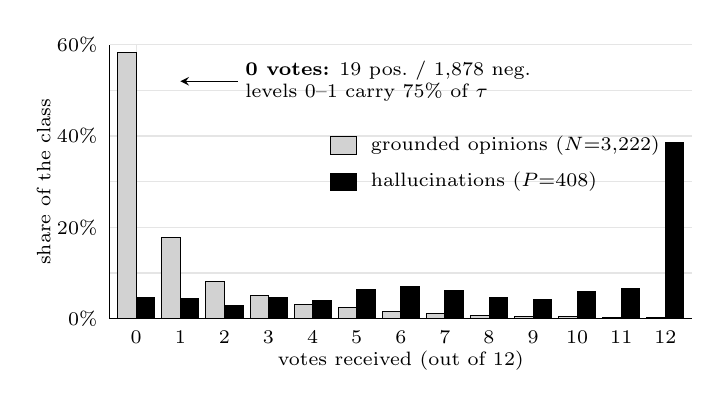
\begin{tikzpicture}[x=0.56cm, y=0.058cm, font=\scriptsize]
  \draw[gray!20] (-0.6,0) grid[xstep=20, ystep=10] (12.6,60);
  \draw (-0.6,0) -- (12.6,0);  \draw (-0.6,0) -- (-0.6,60);
  \foreach \k in {0,...,12} \node[below=1pt] at (\k,0) {\k};
  \foreach \yy in {0,20,40,60} \node[left=1pt] at (-0.6,\yy) {\yy\%};
  \node[below=8pt] at (6,0) {votes received (out of 12)};
  \node[rotate=90] at (-2.1,30) {share of the class};
  % negatives: grey; positives: black
  \foreach \k/\h in {0/58.3,1/17.8,2/8.1,3/5.1,4/3.2,5/2.5,6/1.6,7/1.1,8/0.8,9/0.5,10/0.4,11/0.2,12/0.3}
    \draw[fill=gray!35, line width=0.3pt] (\k-0.42,0) rectangle (\k,\h);
  \foreach \k/\h in {0/4.7,1/4.4,2/2.9,3/4.7,4/3.9,5/6.4,6/7.1,7/6.1,8/4.7,9/4.2,10/5.9,11/6.6,12/38.5}
    \draw[fill=black, line width=0.3pt] (\k,0) rectangle (\k+0.42,\h);
  \node[anchor=west, align=left, inner sep=1pt] at (2.4,52)
    {\textbf{0 votes:} 19 pos.\ / 1,878 neg.\\
     levels 0--1 carry $75\%$ of $\tau$};
  \draw[->, >=stealth] (2.3,52) -- (1.0,52);
  \fill[gray!35, draw=black, line width=0.3pt] (4.4,36) rectangle (5.0,40);
  \node[anchor=west] at (5.1,38) {grounded opinions ($N{=}3{,}222$)};
  \fill (4.4,28) rectangle (5.0,32);
  \node[anchor=west] at (5.1,30) {hallucinations ($P{=}408$)};
\end{tikzpicture}
\caption{The committee's tie structure. For each of the thirteen vote levels,
the share of grounded opinions (grey) and of hallucinations (black) receiving
that many votes. The tie fraction is $\tau=\sum_k \pi^+_k\pi^-_k$, the sum of
products of the two bars at each level: level~0 alone contributes $58\%$ of it
($\pi^-_0=0.583$, $\pi^+_0=0.047$), levels~0--1 contribute $75\%$.}
\label{fig:comite}
\end{figure}

Figure~\ref{fig:comite} explains why the tie fraction is small although half
of the opinions receive zero votes (Example~\ref{ex:comite}). The tie
fraction is a sum of \emph{products} of class shares. The zero-vote class
holds $58\%$ of the grounded opinions but only $4.7\%$ of the hallucinations
($19$ against $1{,}878$ opinions). Hallucinations rarely receive zero votes;
they concentrate at twelve votes ($38.5\%$), where almost no grounded opinion
is found.

\subsection{Decomposing the effect of each combination}
\label{sec:res-mecanismo}

Because AUROC is an average over pairs \eqref{eq:auroc}, it can be decomposed
exactly over any partition of the pairs. We divide the $1{,}314{,}576$
positive--negative pairs into those the committee \emph{separates}
($95.4\%$) and those it \emph{ties} ($4.6\%$), and measure the effect of each
combination on each group (Table~\ref{tab:mecanismo}).

\begin{table}[!ht]
  \centering
  \caption{Exact decomposition of AUROC over pair types.
  ``Reversals'' counts separated pairs whose order the fused score flips:
  \emph{harmful} if the committee had them right, \emph{benign} if wrong.
  One representative fold partition; stability is Table~\ref{tab:estab}.}
  \label{tab:mecanismo}
  \small
  \setlength{\tabcolsep}{5pt}
  \begin{tabular}{@{}lccc ccc@{}}
    \toprule
    & & \multicolumn{2}{c}{\textbf{contribution from}} &
      \multicolumn{3}{c}{\textbf{reversals among separated pairs}} \\
    \cmidrule(lr){3-4}\cmidrule(lr){5-7}
    \textbf{Method} & \textbf{AUROC} & separated & tied &
      total & harmful & benign \\
    \midrule
    committee (vote count) & 0.9260 & 0.9027 & 0.0232 & --- & --- & --- \\
    stacking (logistic)  & 0.9262 & 0.9013 & 0.0249 &
      \textbf{1.33\%} & 0.74\% & 0.59\% \\
    \textbf{lexicographic} & \textbf{0.9300} & 0.9027 & \textbf{0.0272} &
      \textbf{0.00\%} & 0.00\% & 0.00\% \\
    \bottomrule
  \end{tabular}
\end{table}

Tied pairs contribute exactly $\tau/2 = 0.0232$ to the committee's AUROC, as
Lemma~\ref{lem:contab} requires. The weighted combination (``stacking'')
extracts information from them, raising their contribution to $0.0249$
($+0.0017$), but it also reverses $1.33\%$ of the separated pairs, which costs
$0.0014$, so the net gain is $0.0002$. The lexicographic combination reverses
no pair and raises the contribution of the tied pairs to $0.0272$ ($+0.0040$).
The two methods use the same information; they differ only in whether they
may overturn the committee.

\subsection{Main comparison}
\label{sec:res-principal}

\begin{table}[!ht]
  \centering
  \caption{AUROC over twenty independent \texttt{GroupKFold} partitions. The
  reference, the committee's vote count ($0.9260$), does not depend on the
  folds. ``Features'' denotes the speaker-incidence features, including NLI; ``all'' adds
  the structural features of Section~\ref{sec:negativos}. The last column
  gives the share of partitions in which the combination exceeds the
  committee.}
  \label{tab:estab}
  \small
  \begin{tabular}{@{}lrrrr@{}}
    \toprule
    \textbf{Combination} & \textbf{median} & \textbf{min} & \textbf{max} &
      \textbf{$>$ committee} \\
    \midrule
    stacking (committee $+$ features) & 0.9247 & 0.9189 & 0.9276 & 5\% \\
    stacking (committee $+$ all)      & 0.9218 & 0.9173 & 0.9248 & 0\% \\
    committee, out-of-fold weights    & 0.9226 & 0.9175 & 0.9245 & 0\% \\
    \textbf{lexicographic (committee, features)} & \textbf{0.9301} & 0.9295 & 0.9307 & \textbf{100\%} \\
    lexicographic (committee, all)    & 0.9302 & 0.9296 & 0.9306 & \textbf{100\%} \\
    \bottomrule
  \end{tabular}
\end{table}

Table~\ref{tab:estab} supports two conclusions. First, stacking is worse than
the committee in median, and it is unstable: its result varies by $0.0087$
depending only on the fold assignment, a range that includes the committee's
value, so a single run may report either a gain or a loss. Second, the
lexicographic combination varies by $0.0012$, seven times less, and always
exceeds the committee. The paired comparisons on a fixed partition, with
hearing-clustered bootstrap, are:

\begin{center}\small
\begin{tabular}{@{}lcc@{}}
\toprule
\textbf{Comparison} & $\Delta\,\AUC$ & \textbf{95\% CI} \\
\midrule
lexicographic vs.\ committee (vote count)    & $+0.0040$ & $[+0.0005, +0.0078]$ \\
lexicographic vs.\ committee (OOF weights) & $+0.0054$ & $[+0.0005, +0.0105]$ \\
lexicographic vs.\ stacking                & $+0.0067$ & $[+0.0015, +0.0125]$ \\
\bottomrule
\end{tabular}
\end{center}

\subsection{The gain at each level of cost}
\label{sec:res-escada}

Table~\ref{tab:scoreboard2} applies the lexicographic combination to
committees of $1$, $3$, $5$, $8$ and $12$ judges. The rule improves every
committee size, and its gain decreases as the committee grows, as
Equation~\eqref{eq:captura} implies: larger committees tie fewer pairs. The
gain is largest at a single judge call. Every one of the twelve judges
improves, by $+0.046$ to $+0.102$, with all twelve hearing-clustered
intervals excluding zero; a typical judge rises from $0.807$ to $0.881$, and
recovers about $60\%$ of the difference between one judge and the full
committee. The additional cost is ten calls to a small NLI model; without
them the typical gain is still $+0.069$. With more judges the medians in
Table~\ref{tab:scoreboard2} show the same pattern: five judges with the rule
($0.923$) are above eight without it ($0.921$). In a paired comparison,
the median seven-judge subset with the rule differs from the full committee
of twelve by $+0.0001$ (CI $[-0.0046,+0.0049]$), so the two are
statistically indistinguishable. These comparisons are exploratory. On this
dataset, a small committee combined with the rule therefore approaches the
accuracy of a much larger one.

\begin{table}[!ht]
  \centering
  \caption{AUROC by number of LLM judge calls per opinion. For $k$ judges,
  values are medians over $60$ random subsets of $k$ judges (the single full
  committee for $k=12$) on one fold partition. ``Alone'' is the vote count of
  the subset; the next two columns add lexicographic tie-breaking with the
  speaker-incidence features, without and with the ten NLI calls. In the
  first row, ``alone'' is the global-cosine baseline and the features are
  used as the detector. The gain is that of the last column over the first.
  Values differ from Table~\ref{tab:orador} in the third decimal because of
  the fold partition. Script \texttt{j9\_teto.py}.}
  \label{tab:scoreboard2}
  \small
  \begin{tabular}{@{}lcccc@{}}
    \toprule
    & & \multicolumn{2}{c}{\textbf{with tie-breaking}} & \\
    \cmidrule(lr){3-4}
    \textbf{Judge calls} & \textbf{alone} & \textbf{0 NLI calls} &
      \textbf{10 NLI calls} & \textbf{gain} \\
    \midrule
    0  & 0.5676 & 0.7617 & 0.7784 & $+0.2108$ \\
    1  & 0.8067 & 0.8759 & \textbf{0.8806} & $+0.0739$ \\
    3  & 0.8917 & 0.9102 & 0.9121 & $+0.0204$ \\
    5  & 0.9128 & 0.9212 & 0.9230 & $+0.0102$ \\
    8  & 0.9205 & 0.9255 & 0.9272 & $+0.0067$ \\
    12 & 0.9260 & 0.9290 & \textbf{0.9301} & $+0.0041$ \\
    \bottomrule
  \end{tabular}
\end{table}

\paragraph{Forecasting the gain on unseen hearings.} Equation~\eqref{eq:captura}
is an identity when $\tau$ and $\alpha$ are measured on the same data, so
agreement with the observed gain on those data confirms nothing. To test
whether it forecasts the gain, we split the hearings at random into two
halves. On the first half we fit the secondary detector and measure $\alpha$
with out-of-fold scores; on the second half we compute $\tau$ from the
judges' votes alone, forecast the gain as $\tau(\alpha - \tfrac12)$, and compare
it with the gain actually observed there, where the secondary detector was
never fitted. Table~\ref{tab:previsao} reports the results over $50$ random
splits, with a random subset of judges in each. The forecast is essentially
unbiased at every committee size, and it predicts the sign of the gain in
$99\%$ of the $250$ cases. The same forecast computed with the global AUROC
of the secondary detector instead of $\alpha$ overestimates the gain by a factor
of $1.4$ to $3$, as Remark~\ref{rem:orcamento} anticipates. Since $\tau$ is
known from the votes alone and $\alpha$ can be estimated on a small development
set, the gain of the rule can be estimated before it is deployed.

\begin{table}[!ht]
  \centering
  \caption{Forecasting the gain of the lexicographic combination on unseen
  hearings: means over $50$ random splits of the hearings into two halves.
  The forecast uses $\tau$ from the votes of the second half and $\alpha$ (or
  the global AUROC) of the secondary detector on the first half. MAE is the
  mean absolute error of the forecast. Script \texttt{j13\_previsao.py}.}
  \label{tab:previsao}
  \small
  \begin{tabular}{@{}lccccc@{}}
    \toprule
    & & \multicolumn{2}{c}{\textbf{forecast with $\alpha$}} &
      \multicolumn{2}{c}{\textbf{with global AUROC}} \\
    \cmidrule(lr){3-4}\cmidrule(lr){5-6}
    \textbf{Judges} & \textbf{observed gain} & mean & MAE & mean & MAE \\
    \midrule
    1  & $+0.0721$ & $+0.0706$ & $0.0108$ & $+0.1000$ & $0.0279$ \\
    3  & $+0.0284$ & $+0.0270$ & $0.0083$ & $+0.0490$ & $0.0206$ \\
    5  & $+0.0152$ & $+0.0148$ & $0.0062$ & $+0.0310$ & $0.0159$ \\
    8  & $+0.0075$ & $+0.0073$ & $0.0044$ & $+0.0185$ & $0.0111$ \\
    12 & $+0.0042$ & $+0.0041$ & $0.0032$ & $+0.0130$ & $0.0088$ \\
    \bottomrule
  \end{tabular}
\end{table}

\paragraph{The gain expressed in judge calls.} Over twenty fold partitions and
sixty random subsets of judges per subset size, eight judges combined
lexicographically with the features reach $0.9272$, against $0.9260$ for the
full twelve-judge committee. The difference, $+0.0008$ (CI
$[-0.0031,+0.0048]$), is non-inferior at a margin of $0.0040$, the size of the
effect claimed in this paper. The combination matches or exceeds the full
committee in $73\%$ of the eight-judge subsets and in $97\%$ of the nine-judge
subsets. In this exploratory analysis, eight or nine judges combined with the
features therefore match the full committee in most random subsets, which
would save three to four judge calls per opinion. Two limitations apply. The choice of judges matters more
than the fold assignment (standard deviation $0.0025$ across subsets against
$0.0004$ across folds, at seven judges), so a correlated choice, such as four
models with the same prompt, performs worse than a random one. With seven
judges or fewer, the shortfall exceeds the margin. This analysis is
exploratory.

\paragraph{Individual judges.} Applied to each judge separately, the
lexicographic combination outperforms stacking for all twelve judges, six of
them with clustered CIs excluding zero, and the largest gains go to the
judges with the most ties. The headline single-call figures of this paper are
those of a typical judge (Table~\ref{tab:scoreboard2}); the best judge is a
variant selected after the fact. For that judge (\texttt{p2\_gpt4omini},
$0.8468$), the combination reaches $0.8928$, against $0.8877$ with stacking;
adding the structural features of Section~\ref{sec:negativos} gives
$0.8942$.

\paragraph{Where the combination is useful.} Both $\tau$ and $\alpha$ depend on
how coarse the primary detector is. The best single judge (AUROC $0.8468$)
ties $\tau = 26.1\%$ of the pairs, a maximum gain of $0.1307$, which is $5.6$
times that of the twelve-judge committee. On these ties the
speaker-incidence features reach $\alpha = 0.676$, against $0.5856$ on the
committee's ties. Equation~\eqref{eq:captura} accounts exactly for the observed
gains, $+0.0460$ ($0.8468 \to 0.8928$) and $+0.0040$ ($0.9260 \to 0.9300$).
The gain is eleven times larger with one judge than with twelve, and the
maximum gain $\tau/2$, which is known from the judges' votes alone, already
indicates this.



\subsection{How much of the possible gain is obtained, and why not more}
\label{sec:res-orcamento}

Equation~\eqref{eq:captura} expresses the observed gain as a property of the
secondary detector. On the representative partition, the speaker-incidence
features reach $\alpha = 0.5856$ on the committee's ties (median $0.589$ over
twenty partitions), so the combination recovers $2\alpha - 1 \approx 17\%$ of
the maximum gain $\tau/2$. The value $\tau(\alpha - \tfrac12)$ equals the
observed $+0.0040$; we verified the identity numerically to six decimal
places.
Table~\ref{tab:anatomia} shows how this value arises.

\begin{table}[!ht]
  \centering
  \caption{AUROC of the speaker-incidence features on each group of pairs,
  by what the committee does with the pair; medians over twenty fold
  partitions. The middle row is the maximum gain of
  Proposition~\ref{thm:lex}(iii). The last row limits everything else: where the
  committee is wrong, the features are wrong as well.}
  \label{tab:anatomia}
  \small
  \begin{tabular}{@{}lrrc@{}}
    \toprule
    \textbf{the committee\ldots} & \textbf{\% of pairs} &
      \textbf{contributes} & \textbf{features' AUROC} \\
    \midrule
    separates, correctly        & 90.3\% & 0.9027 & 0.809 \\
    \textbf{ties}               &  4.6\% & \textbf{0.0232} & \textbf{0.589} \\
    separates, \textbf{wrongly} &  5.1\% & 0.0000 & \textbf{0.473} \\
    \bottomrule
  \end{tabular}
\end{table}

The maximum gain is highly concentrated (Figure~\ref{fig:comite}). Three
quarters of it depends on the $37$ hallucinations ($19+18$) that received
zero or one vote. These are, by construction, the hardest cases in the
dataset, since eleven or twelve judges did not flag them, and only $19$ of
them lie in the zero-vote class, against $1{,}878$ grounded opinions. On these
cases the features reach $\alpha = 0.56$; where they perform well ($0.87$ at
twelve votes), only $2.3\%$ of the maximum gain is available. The structural
features of Section~\ref{sec:negativos} change $\alpha$ from $0.5856$ to
$0.5852$.

\paragraph{Limits of the remaining gap.} The features reach $0.809$ on the
pairs the committee orders correctly, $0.589$ on the pairs it ties, and
$0.473$, below chance, on the pairs it orders incorrectly; the last value
never exceeds $0.482$ across twenty partitions. The features therefore agree
with the committee precisely where the committee is wrong. This limits both
remaining sources of gain. Ordering the ties can recover only what
$\alpha = 0.589$ allows, and no rule that overrules the committee when the
features are confident can recover the $0.0508$ of AUROC lost to the
committee's incorrect orderings, since disagreement with the committee is
not a sign of committee error. Table~\ref{tab:mecanismo} shows
the same effect: only $44\%$ of the pairs that stacking reversed were in the
wrong order.

We tested this conclusion directly. Six pre-specified attempts to raise
$\alpha$ (fitting the secondary detector within each committee class, adding the
vote count as a feature, interactions with the vote count, interactions with
four coarse strata, weighting by the mass of tied pairs, and a pairwise
ranking loss on the tied pairs only) all \emph{lower} it, from a median of
$0.589$ to between $0.489$ and $0.520$, in all twenty fold partitions. The
limit is not due to the model class either: gradient-boosted trees on the
votes and all features reach $0.9042$, below the committee alone. One of these
failures yields a practical rule: \emph{the secondary detector should not
receive the primary detector's output as input}. With the vote count as a
feature, the secondary detector's global AUROC rises to $0.9260$, because it
relearns the committee, while its $\alpha$ falls to $0.514$. The norm of its
speaker-incidence coefficients halves ($0.921 \to 0.470$) and their direction
rotates (cosine $0.889$). Since the vote count is constant within a tied
class, only this rotated and weaker direction remains to order the ties.

Finally, the combinations $f_\gamma$ of Remark~\ref{rem:portao}, which allow
the secondary detector to move an item across up to $\gamma$ classes of the
committee, do not help with the actual features: $\gamma = 2$ exceeds the
lexicographic combination by only $+0.0005$ (CI $[-0.0004,+0.0013]$) and
exceeds its median in $85\%$ of the twenty partitions, while giving up the
guarantee of Proposition~\ref{thm:lex}(i). The mechanism is not the limitation:
with a perfect secondary detector, $f_\gamma$ ranges from $0.9492$ to $0.9975$
as $\gamma$ grows. To estimate how good a new feature would need to be, we
replaced the secondary detector by the true label, flipped at random for a
fraction $\rho$ of the opinions, and for each $\rho$ between $0$ and $0.5$
searched for a value of $\gamma$ at which $f_\gamma$ outperforms the
lexicographic combination. Overruling the committee helps only while the
detector's AUROC on the committee's incorrectly ordered pairs exceeds
approximately $0.58$.\footnote{Script \texttt{j10\_portao.py}; the value is
interpolated between the tested levels of $\rho$.} The speaker-incidence
features reach $0.473$ on those pairs.

\subsection{Effect on a human review queue}
\label{sec:res-fila}

AUROC concerns pairs of opinions, whereas a human reviewer works through a
queue, from the most to the least suspect opinion, until the review budget is
exhausted. Figure~\ref{fig:fila} reports, for each detector, the share of the
$408$ hallucinations found when the top $k\%$ of opinions are sent to a human
reviewer.

\begin{figure}[!ht]
\centering
% Coordinates generated by codigo/j11_operacao.py, section (7). Do not edit
% by hand: rerun the script and paste.
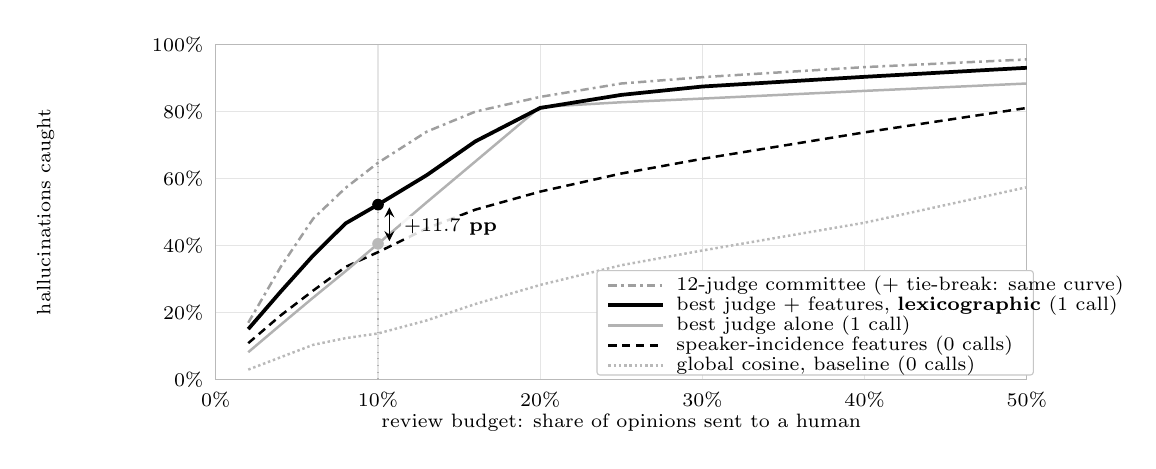
\begin{tikzpicture}[x=0.206cm, y=0.0425cm, font=\scriptsize,
                    c/.style={line width=0.9pt, line join=round},
                    comite/.style={c, gray!75, dash pattern=on 3pt off 1.5pt on 1pt off 1.5pt},
                    jlex/.style={c, line width=1.35pt},
                    juiz/.style={c, gray!60},
                    fam/.style={c, densely dashed},
                    cosg/.style={c, gray!55, densely dotted}]
  \draw[gray!20] (0,0) grid[xstep=10, ystep=20] (50,100);
  \draw[gray!55] (0,0) rectangle (50,100);
  \foreach \x in {0,10,20,30,40,50} \node[below=1pt] at (\x,0) {\x\%};
  \foreach \yy in {0,20,40,60,80,100} \node[left=1pt] at (0,\yy) {\yy\%};
  \node[below=9pt] at (25,0) {review budget: share of opinions sent to a human};
  \node[rotate=90] at (-10.5,50) {hallucinations caught};
  \draw[gray!60, dotted] (10,0) -- (10,66);
  \draw[cosg] plot coordinates {(2,2.9) (4,6.6) (6,10.3) (8,12.3) (10,13.7) (13,17.6) (16,22.5) (20,28.2) (25,34.1) (30,38.5) (40,46.8) (50,57.4)};
  \draw[fam] plot coordinates {(2,10.8) (4,19.1) (6,26.5) (8,33.6) (10,38.0) (13,45.1) (16,50.7) (20,56.1) (25,61.5) (30,65.9) (40,73.8) (50,81.1)};
  \draw[juiz] plot coordinates {(2,8.1) (4,16.3) (6,24.4) (8,32.3) (10,40.5) (13,52.9) (16,65.1) (20,81.4) (25,82.8) (30,83.9) (40,86.2) (50,88.4)};
  \draw[jlex] plot coordinates {(2,15.0) (4,26.2) (6,37.0) (8,46.6) (10,52.2) (13,61.0) (16,71.1) (20,81.1) (25,85.0) (30,87.5) (40,90.4) (50,93.1)};
  \draw[comite] plot coordinates {(2,16.9) (4,33.6) (6,48.0) (8,57.2) (10,64.7) (13,74.0) (16,80.0) (20,84.4) (25,88.4) (30,90.3) (40,93.3) (50,95.6)};
  \fill (10,52.2) circle (2.1pt); \fill[gray!55] (10,40.5) circle (2.1pt);
  \draw[<->, >=stealth, line width=0.6pt] (10.7,41.3) -- (10.7,51.4);
  \node[anchor=west, inner sep=1pt, fill=white, fill opacity=0.85,
        text opacity=1] at (11.4,45.5) {\textbf{$+11.7$ pp}};
  % legend
  \begin{scope}[shift={(24.2,2.5)}]
    \draw[fill=white, draw=gray!45, rounded corners=1pt] (-0.7,-1.2) rectangle (26.2,30);
    \draw[comite] (0,25.6) -- (3.4,25.6);
      \node[anchor=west, inner sep=1.5pt] at (3.9,25.6) {12-judge committee ($+$ tie-break: same curve)};
    \draw[jlex]   (0,19.6) -- (3.4,19.6);
      \node[anchor=west, inner sep=1.5pt] at (3.9,19.6) {best judge $+$ features, \textbf{lexicographic} (1 call)};
    \draw[juiz]   (0,13.6) -- (3.4,13.6);
      \node[anchor=west, inner sep=1.5pt] at (3.9,13.6) {best judge alone (1 call)};
    \draw[fam]    (0,7.6) -- (3.4,7.6);
      \node[anchor=west, inner sep=1.5pt] at (3.9,7.6) {speaker-incidence features (0 calls)};
    \draw[cosg]   (0,1.6) -- (3.4,1.6);
      \node[anchor=west, inner sep=1.5pt] at (3.9,1.6) {global cosine, baseline (0 calls)};
  \end{scope}
\end{tikzpicture}
\caption{Share of hallucinations found as a function of the review budget.
The curve of the best judge alone is a straight line up to $20\%$: a binary
verdict does not order the opinions within each of its two classes, so the
queue is in random order there. Ordering these ties with the
speaker-incidence features adds $11.7$ percentage points at a $10\%$ budget
with one judge call; with twelve judges the difference is not measurable.}
\label{fig:fila}
\end{figure}

At the inexpensive levels, the operational gain is large and agrees with the
theory. When one opinion in ten is reviewed, the global-cosine baseline finds
$13.7\%$ of the hallucinations, the speaker-incidence features $38.0\%$ at
the same zero cost, and a single judge combined with them $52.2\%$, against
$40.5\%$ for the same judge alone. This single-judge gap follows from
Equation~\eqref{eq:captura} with $\tau = 26.1\%$: a binary judge ties most
pairs, so most of its queue is unordered.

With twelve judges, however, the gain in the queue is not measurable. We
predicted in advance that the lexicographic queue would outperform the committee's
at every review budget. It does not: the differences are $-0.2$, $+0.3$ and
$+0.6$ percentage points at budgets of $5\%$, $10\%$ and $20\%$, and every
hearing-clustered interval includes zero. The committee's own queue is
ambiguous, since its thirteen levels leave the achievable recall within an
interval of $1.7$ to $4.7$ points, so two reviewers with the same committee
and budget may not review the same opinions. This ambiguity is small,
however, and a gain of $\tau/2 = 0.0232$ in AUROC is too small and too spread
out to change a review budget. At twelve judges the result is therefore a
ranking improvement, not a workload improvement; at one judge it is both.

\subsection{Controls}
\label{sec:res-controles}

\textbf{Random tie-breaking.} Ordering the ties at random has the same
expected AUROC as not ordering them, but a non-negligible variance: over
$200$ independent draws the mean is $0.9259$ (standard deviation $0.0020$,
maximum $0.9308$). A single random draw is therefore not an adequate control.
Against this null distribution, the lexicographic result of $0.9300$ has
$p = 0.015$.

\textbf{A weak secondary detector, and the order of the combination.} Using
the global cosine as the secondary detector ($\alpha = 0.5409$) gives $0.9279$,
a difference of $+0.0021$ $[-0.0017,+0.0057]$ that is not significant, as
is consistent with its low $\alpha$ under Equation~\eqref{eq:captura}. The lexicographic
combination is also asymmetric by design: the committee comes first because
it is the more reliable detector, and reversing the order would lose the
guarantee of Proposition~\ref{thm:lex}(i).

% =============================================================================
\section{Negative Results}
\label{sec:negativos}

This section reports the pre-specified predictions that the data
contradicted. Two others appear in the results: conditioned entailment does
not outperform conditioned cosine similarity (Section~\ref{sec:res-orador}),
and at twelve judges the combination does not improve the review queue
(Section~\ref{sec:res-fila}).

\textbf{Structural features add nothing to the combination.} We built five
features from the relation between opinions and speakers: its homology
\citep{dowker1952homology}, a Hodge decomposition
\citep{jiang2011statistical} of attribution discrepancies, duplication
between opinions, and two constraints on the order and exclusivity of the
support. Individually, each is either uninformative (the relation has no
cycles in any hearing; the constraints are already satisfied by $87$ to
$93\%$ of the opinions) or redundant with the speaker-incidence features.
Together they raise the zero-cost detector from $0.7611$ to $0.7718$
(paired $+0.0107$, CI $[+0.0012,+0.0205]$), but they leave the combination
with the committee unchanged ($0.9302$ median in both cases). The gain
reported in this paper is due to the combination rule, not to these
features.

\textbf{Attempts to improve the secondary detector on the ties fail.}
Fitting the secondary detector separately within each committee class gives
$0.9237$, below a single global model, because the class that holds most of
the maximum gain contains only $19$ positives. This and the five other
pre-specified attempts described in Section~\ref{sec:res-orcamento} all lower
$\alpha$.

% =============================================================================
\section{Threats to Validity}
\label{sec:ameacas}

\paragraph{Labels.} The hallucination labels are those released with
PublicHearingBR \citep{publichearingbr}, which we use as given; our
conclusions are conditional on their quality, and no inter-annotator
agreement is available for them. The audit of Section~\ref{sec:auditoria}
characterises the positives but does not replace the labels.

\paragraph{Binary judges.} The judges' votes are binary, so the maximum gain
$\tau/2$ would shrink if the judges produced calibrated probabilities. Our
result on combination is conditional on this format.

\paragraph{Speaker recovery.} Speakers are matched by name for $85.7\%$ of
the opinions, and matching errors are not necessarily conservative: excluding
the hearings with deaf participants, whose turns read \emph{``(Manifestação
em LIBRAS.)''} while the content appears in the interpreter's voice ($1.1\%$
of the opinions), lowers the main signal from $0.7455$ to $0.7314$. All
entailment probabilities come from a single multilingual NLI model.

\paragraph{Scope of the claims.} The gain over the full committee is small
($+0.0040$, clustered CI lower bound $+0.0005$) and rests on its consistency:
it holds in all twenty fold partitions and for all twelve individual judges
($p=0.015$ against random tie-breaking). The share of partitions measures
stability on a fixed dataset, not replication. The advantage over stacking
($+0.0067$) is more robust. The confirmatory comparisons are the three of
Section~\ref{sec:res-principal} and the six attempts to raise $\alpha$; the
per-judge results, Table~\ref{tab:scoreboard2} (one fold partition, medians
over random subsets of judges), the decomposition of
Section~\ref{sec:res-orcamento} and the audit are exploratory.

% =============================================================================
\section{Conclusion}
\label{sec:conclusao}

Verification scores that pool sentence-level similarity or entailment over a
whole transcript cannot, in principle, tell whether an opinion was expressed
by the person to whom it is attributed. On PublicHearingBR, conditioning on
the attributed speaker's turns raises the AUROC of an inexpensive detector
from $0.57$ to $0.76$ without any model call, and improves each of the twelve
LLM judges. An audit of 50 positives indicates that about a quarter of them
are misattributions of this kind.

Adding such a detector to a committee of judges requires care. Fitting a
single model on both reverses some of the committee's decisions, and on this
dataset it cancels the benefit. Ranking by the committee and using the
inexpensive detector only to order its ties never reverses a decision, and its
gain is given exactly by the tie fraction and by the detector's AUROC on the
tied pairs. The tie fraction, known from the judges' votes alone, bounds the
gain and indicates where the combination is useful. The main practical
consequence is a large reduction in cost. With a single judge call, the rule
raises every judge's AUROC, a typical judge from $0.81$ to $0.88$, which
recovers about $60\%$ of the difference to the full committee;
when a reviewer checks the $10\%$ most suspect opinions, the share of
hallucinations found rises from $40.5\%$ to $52.2\%$. In an exploratory analysis, seven judges with the rule are statistically
indistinguishable from the full committee of twelve, and the full committee
itself improves from $0.926$ to $0.930$. Because the gain decomposes into two
quantities that can be measured in advance, it can also be forecast on new
data, which we verified on held-out hearings. The remaining gap cannot be closed with these
features, since they perform below chance on the pairs that the committee
orders incorrectly.

Several predictions failed,
and we report them alongside the results that held. The proofs use only the rankings
induced by the scores, so the results apply to any primary and secondary
detector and can be checked on a new deployment by counting pairs.

\medskip\noindent\textbf{Reproducibility.} All numbers in this paper are
produced by the scripts in the \texttt{codigo/} directory of the public
repository (\url{https://github.com/caua-sathler/IdeiasEmRede-TopoIA}),
together with the prediction files written before each experiment. The
pipelines use cached intermediate results and fixed random seeds, and each runs
in minutes on a single laptop with 8\,GB of memory. We thank Instituto Kunumi
for the \emph{Ideias em Rede} challenge, the authors of PublicHearingBR for
the corpus and the judge annotations, and the DCC/UFMG course infrastructure.

% =============================================================================
% Referencias em 8pt (o padrao de templates de conferencia IEEE/ACM), para
% caber no limite de 15 paginas sem reduzir corpo de texto, tabelas ou figuras.
\begingroup
\scriptsize
\setlength{\bibsep}{0pt plus 0.2ex}
\bibliography{referencias}
\endgroup

% =============================================================================
\end{document}
